\chapter{Il percorso di stage }\label{cap:Il_percorso}
\section{Formazione}
Il processo di formazione ha avuto un ruolo fondamentale nella buona riuscita del progetto di stage, con una durata complessiva di circa quattro settimane. \\
La causa del protrarsi del processo di formazione è stata provocata dalla mia inesperienza in merito a 
concetti legati all'architettura \gls{eda}{},
\textbf{Apache Kafka}, \textbf{Apache Druid} e \textbf{Docker Compose}.\\  
Tutto il processo di formazione è stato tracciato e monitorato da me medesimo e dal tutor aziendale attraverso le \gls{board}{} offerte 
dal software di \gls{project management}{} \textbf{ClickUp} (Figura \ref{cap:ClickUp}).\\
\begin{figure}[h]
    \centering
    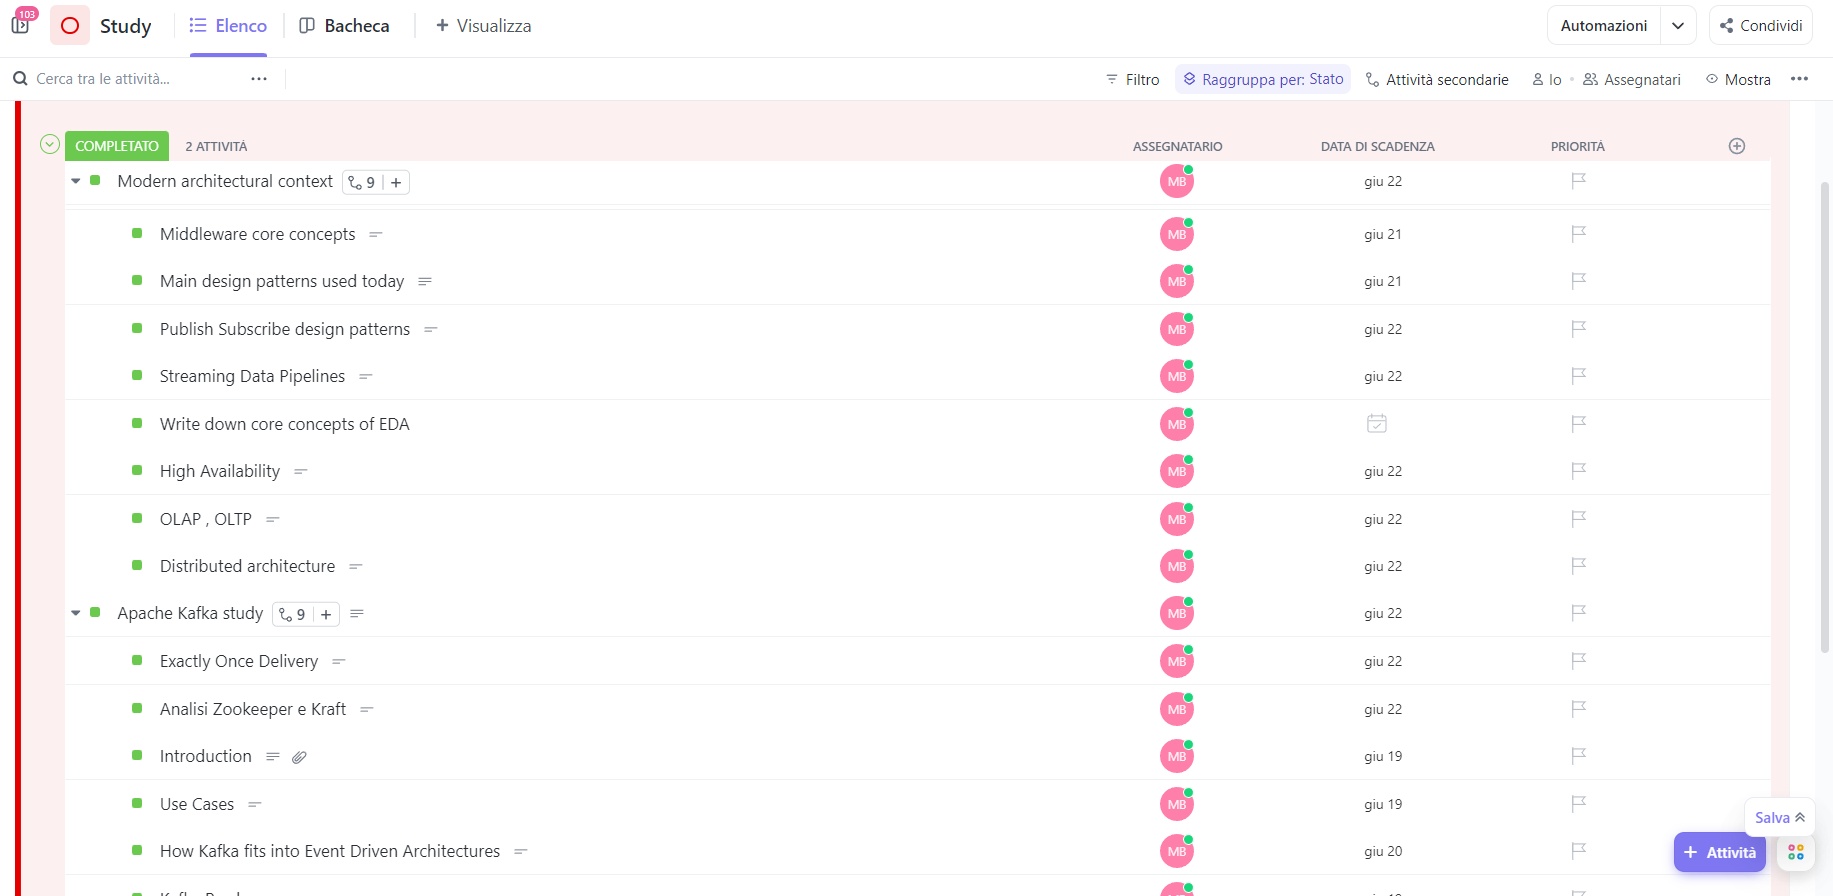
\includegraphics[width=1\textwidth]{images/percorso/formazione.png}
    \caption{Board di ClickUp per il processo di formazione}
    \label{cap:ClickUp}
\end{figure}
\pagebreak
\\
Inoltre durante il processo di formazione, oltre a reperire informazioni da documentazione ufficiale, ho avuto anche modo 
di approfondire quanto appena appreso attraverso delle attività di \gls{hands-on}{} che mi hanno permesso di mettere in pratica nell'immediato quanto appreso
(Figura \ref{cap:Hands-on}).
\begin{figure}[h]
    \centering
    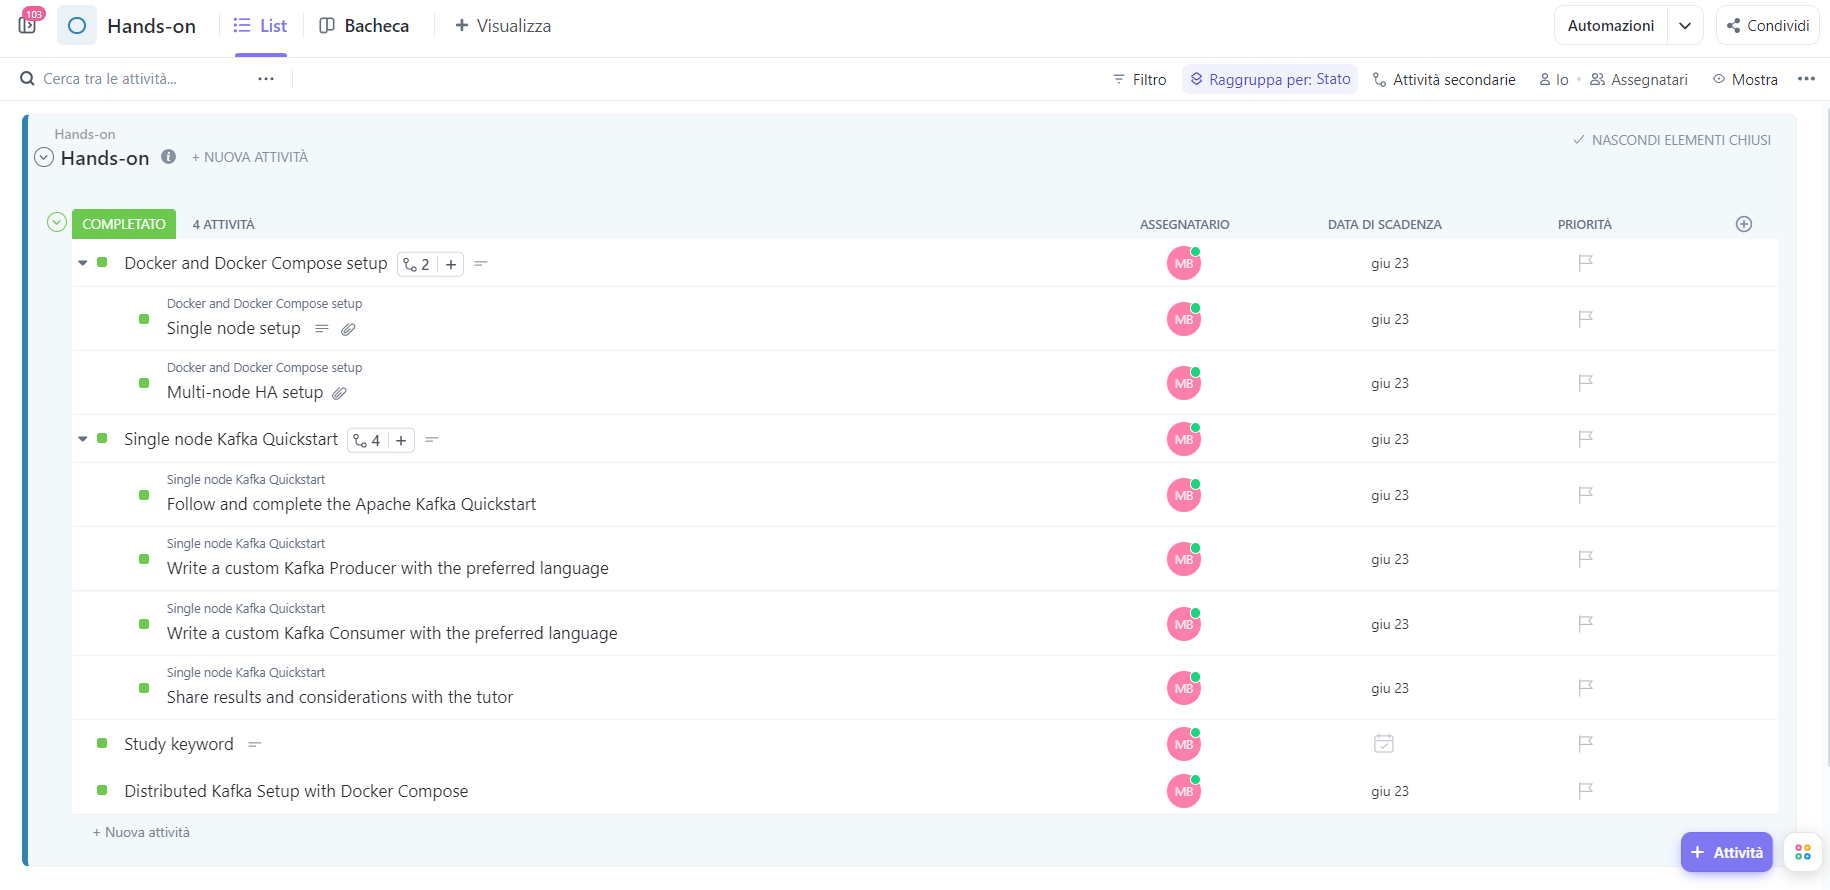
\includegraphics[width=1\textwidth]{images/percorso/hands_on.png}
    \caption{Attività di hands-on per il processo di formazione}
    \label{cap:Hands-on}
\end{figure}
\\
Inoltre durante il processo di formazione, in collaborazione con il tutor aziendale, è stato definito anche un processo di coordinamento e produzione di 
documentazione che mi ha permesso, durante tutto lo svolgimento del percorso di stage, di avere un tracciamento dei concetti appresi,
 di avere un eventuale riferimento per un'eventuale risoluzione di problemi o dubbi sorti (Figura \ref{cap:Documentazione}).
\begin{figure}[h]
    \centering
    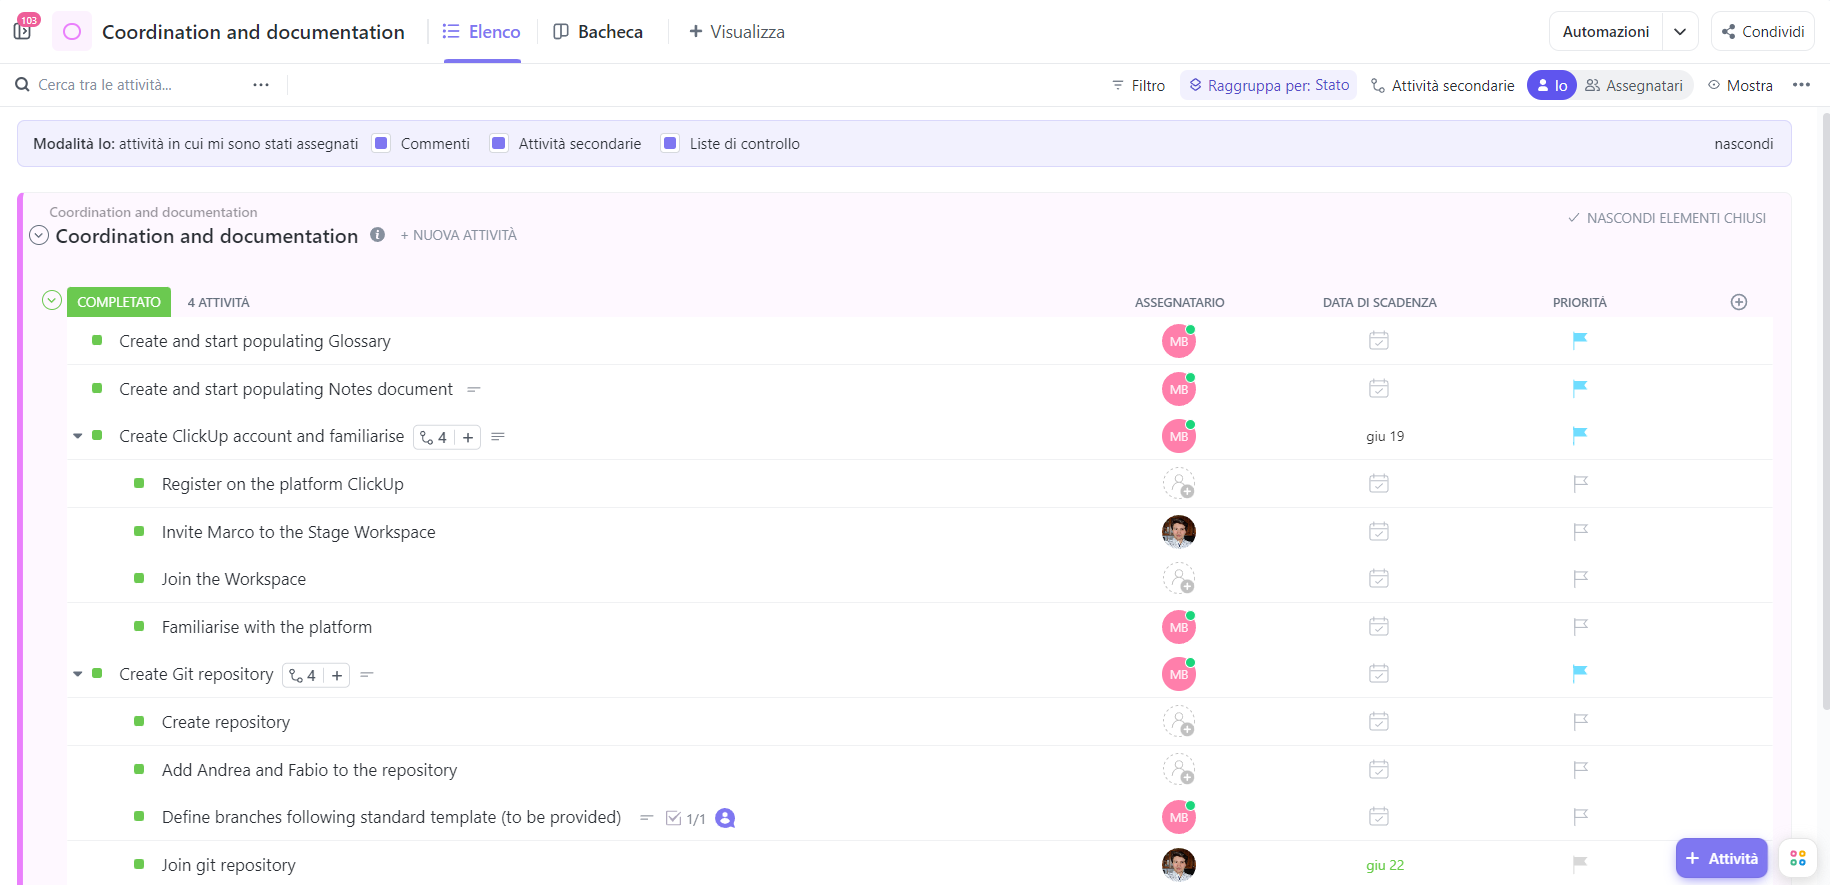
\includegraphics[width=1\textwidth]{images/percorso/coordinamento.png}
    \caption{Board di ClickUp per il processo di coordinamento e documentazione}
    \label{cap:Documentazione}
\end{figure}
\subsection{Daily stand-up meeting}
In ausilio dei processi sopra descritti, 
è stato anche definito, in concomitanza con l'inizio del processo di formazione, un processo di \textbf{supporto} ispirato al metodo \gls{Scrum}{}, 
andando a programmare degli incontri giornalieri di circa 15 minuti finalizzati a:
\begin{list}{*}
    \item \textbf{monitorare} lo stato di avanzamento delle attività svolte, da svolgere e in corso di svolgimento;
    \item \item \textbf{risolvere} eventuali dubbi o problemi sorti durante lo svolgimento delle attività;
    \item \textbf{definire} eventuali miglioramenti o cambiamenti da apportare alle da svolgere, o in corso di svolgimento, e al metodo 
    di lavoro adottato.
\end{list}
\section{Codifica}
\subsection{Configurazione di un cluster Kafka con Docker Compose}
Dopo aver terminato le attività di formazione su \textbf{Apache Kafka} e \textbf{Docker Compose} 
ho iniziato la configurazione di un \gls{cluster}{}, che fa uso di \gls{container}{}, in grado di testare tali strumenti.
\\Seguendo la buona pratica dell'alta affidabilità, descritta del 
paragrafo \ref{sec:alta_affidabilita}, ho configurato un \gls{cluster}{} con tre nodi \textbf{Kafka} e un nodo \textbf{Zookeeper}.\\
Innanzitutto per far si che ogni \gls{container}{} possa comunicare con gli altri è necessario creare una 
\gls{Docker network}{}, denominata \textbf{kafka-druid}, nel seguente modo.
\begin{lstlisting}[caption=\texttt{docker network create}, label=lst:file]{docker network create}
docker network create kafka-druid
\end{lstlisting}
Successivamente sono stati creati i nodi \textbf{Zookeeper} e \textbf{Kafka} con \textbf{Docker Compose} 
utilizzando il seguente file di 
configurazione (per motivi di spazio viene riportata la definizione di un solo nodo \textbf{Kafka}, la configurazione degli altri è del tutto analoga).
\begin{lstlisting}[caption=\texttt{kafka-cluster-compose.yml}, label=lst:file]{kafka-cluster-compose.yml}
networks:
  kafka-druid:
    name: kafka-druid
    driver: bridge
    external: true
services:
  kafka:
    image: confluentinc/cp-kafka:7.4.0
    hostname: kafka
    container_name: kafka
    networks:
      - kafka-druid
    ports:
      - "29092:29092"
    environment:
      KAFKA_ADVERTISED_LISTENERS: INTERNAL://kafka:9092,EXTERNAL://localhost:29092
      KAFKA_LISTENER_SECURITY_PROTOCOL_MAP: INTERNAL:PLAINTEXT,EXTERNAL:PLAINTEXT
      KAFKA_INTER_BROKER_LISTENER_NAME: INTERNAL
      KAFKA_ZOOKEEPER_CONNECT: "zookeeper:2181"
      KAFKA_BROKER_ID: 1
      KAFKA_LOG4J_LOGGERS: "kafka.controller=INFO,kafka.producer.async.DefaultEventHandler=INFO,state.change.logger=INFO"
      KAFKA_OFFSETS_TOPIC_REPLICATION_FACTOR: 1
      KAFKA_TRANSACTION_STATE_LOG_REPLICATION_FACTOR: 1
      KAFKA_TRANSACTION_STATE_LOG_MIN_ISR: 1
      KAFKA_AUTHORIZER_CLASS_NAME: kafka.security.authorizer.AclAuthorizer
      KAFKA_ALLOW_EVERYONE_IF_NO_ACL_FOUND: "true"

\end{lstlisting}
È importante sottolineare che all'interno della configurazione, sopra descritta, 
vengono utilizzate le \gls{immagini Docker}{} \\\textbf{confluentinc/cp-zookeeper:7.4.0} e \textbf{confluentinc/cp-kafka:7.4.0}.\\
Tale scelta è stata adottata, dal fatto che oramai \textbf{Confluent} 
è diventata una distribuzione molto alla avanguardia, in quanto fornisce soluzioni, utilizzate anche a livello aziendale,
per la gestione di flussi di dati in tempo reale, come in Sync Lab.\\
Nonostante ciò si precisare che per i test che verranno elencati di seguito,
sono utilizzabili anche le \gls{immagini Docker}{} ufficiali di \textbf{Apache Kafka} e \textbf{Apache Zookeeper}, distribuite dalla 
\gls{Apache Software Foundation}.
\subsection{Configurazione del file di enviroment per il cluster di Apache Druid}
Dopo aver configurato il \gls{cluster}{} di \textbf{Apache Kafka}, è stato necessario adattarne il file di \gls{enviroment}{} nel seguente modo.
\begin{lstlisting}[caption=\texttt{enviroment}, label=lst:file]{enviroment}
DRUID_MAXDIRECTMEMORYSIZE=3072m
DRUID_SINGLE_NODE_CONF=nano-quickstart
druid_emitter_logging_logLevel=debug
druid_extensions_loadList=["druid-histogram", "druid-datasketches", "druid-lookups-cached-global", "postgresql-metadata-storage", "druid-multi-stage-query", "druid-kafka-indexing-service"]
druid_zk_service_host=zookeeper
druid_lookup_enableLookupSyncOnStartup=true
druid_lookup_lookupTierIsDatasource=false
druid_lookup_lookupTier=_default_tier
druid_broker_cache_useCache=true
druid_broker_cache_populateCache=true
druid_broker_cache_useResultLevelCache=true
druid_broker_cache_populateResultLevelCache=true
druid_cache_useCache=true
druid_cache_populateCache=true
druid_cache_useResultLevelCache=true
druid_cache_populateResultLevelCache=true
druid_metadata_storage_host=
druid_metadata_storage_type=postgresql
druid_metadata_storage_connector_connectURI=jdbc:postgresql://postgres:5432/druid
druid_metadata_storage_connector_user=druid
druid_metadata_storage_connector_password=FoolishPassword
druid_coordinator_balancer_strategy=cachingCost
druid_indexer_runner_javaOptsArray=["-server", "-Xmx1g", "-Xms1g", "-XX:MaxDirectMemorySize=3g", "-Duser.timezone=UTC", "-Dfile.encoding=UTF-8", "-Djava.util.logging.manager=org.apache.logging.log4j.jul.LogManager"]
druid_indexer_fork_property_druid_processing_buffer_sizeBytes=256MiB
druid_storage_type=local
druid_storage_storageDirectory=/opt/shared/segments
druid_indexer_logs_type=file
druid_indexer_logs_directory=/opt/shared/indexing-logs
druid_processing_numThreads=1
druid_processing_numMergeBuffers=1
DRUID_LOG4J=<?xml version="1.0" encoding="UTF-8" ?><Configuration status="WARN"><Appenders><Console name="Console" target="SYSTEM_OUT"><PatternLayout pattern="%d{ISO8601} %p [%t] %c - %m%n"/></Console></Appenders><Loggers><Root level="info"><AppenderRef ref="Console"/></Root><Logger name="org.apache.druid.jetty.RequestLog" additivity="false" level="DEBUG"><AppenderRef ref="Console"/></Logger></Loggers></Configuration>
\end{lstlisting}
Tale azione è stata resa necessaria dal fatto che \textbf{Apache Druid} è uno strumento \gls{olap}{}, che necessita di grandi quantità di memoria RAM e spazio su disco per operare 
su moli considerevoli di dati.\\
Pertanto si sottolinea, che nella configurazione sopra citata, viene utilizzata una versione di \textbf{Druid}, denominata \textbf{nano-quickstart}, che permette di utilizzare tale strumento con un consumo di risorse ridotto.
\subsection{Configurazione di un cluster di Apache Druid con Docker Compose}
Per definizione del \gls{cluster}{} di \textbf{Apache Druid},
al fine di ottimizzare il consumo di memoria RAM necessaria per la sua esecuzione,
sono stati utilizzati un nodo per ogni processo di \textbf{Apache Druid}.
Nel seguente file di configurazione vengono definiti: un nodo 1\textbf{Coordinator}, \textbf{Historical}, \textbf{Broker} e \textbf{MiddleManager}, implementato per mezzo di \textbf{PostgreSQL}. 
\pagebreak
\begin{lstlisting}[caption=\texttt{druid-cluster-compose.yml}, label=lst:file]{druid-cluster-compose.yml}
volumes:
  coordinator_var: {}
  druid_shared: {}
services:
  coordinator:
    image: apache/druid:26.0.0
    container_name: coordinator
    networks:
      - kafka-druid
    volumes:
      - druid_shared:/opt/shared
      - coordinator_var:/opt/druid/var
    depends_on:
      - zookeeper
      - postgres
    ports:
      - "8081:8081"
    command:
      - coordinator
    env_file:
      - environment
\end{lstlisting}
È importante sottolineare che all'interno del file di configurazione, sopra descritto, vengono definite anche 
i \gls{volumi}{} necessari per l'archiviazione dei dati e dei \gls{log}{}, essenziali al funzionamento del \gls{cluster}{}.
\subsection{Creazione del produttore di eventi Kafka}
AL file di poter testare i \gls{cluster}{} creati, la prima attività di codifica è stata la definizione di
un produttore di eventi \textbf{Kafka} che generasse eventi casuali.\\
Per la creazione del produttore di eventi \textbf{Kafka} è stato utilizzato il linguaggio di programmazione \textbf{Python} e la libreria \gls{Kafka-Python}{}, in particolare il modulo \textbf{KafkaProducer} nel seguente modo:
\begin{lstlisting}[language=Python, caption=\texttt{producer.py}, label=lst:file]{producer.py}
producer = KafkaProducer(  
  bootstrap_servers = ['localhost:29092'],  
  value_serializer = lambda x:json.dumps(x).encode('utf-8')  
  )  
\end{lstlisting}
È importante sottolineare che il produttore \textbf{Kafka} è stato creato in modo tale da inviare gli eventi, al relativo \gls{topic}{} di appartenenza, in formato \gls{json}{}.
 in formato \gls{json}{} alla porta pubblica 
del nodo \textbf{Kafka} precedentemente configurato, unica porta che può essere raggiunta dall'esterno.\\
\pagebreak
\section{Esecuzione e testing}
\subsection{Creazione di una Data Pipeline}
Dopo aver ultimato la configurazione dei \gls{cluster}{} \textbf{Apache Kafka} e \textbf{Apache Druid} con \textbf{Docker Compose} 
e aver creato il produttore di eventi \textbf{Kafka}, è stato possibile creare una \textbf{Data Pipeline} che permettesse d'inviare gli eventi generati dal produttore \textbf{Kafka} al \gls{cluster}{} di \textbf{Apache Kafka} e 
successivamente effettuare l'\gls{injection}{} all'interno del \gls{cluster}{} di \textbf{Apache Druid} per effettuare il \gls{Data Processing}.
\subsubsection{Confronto delle prestazioni di esecuzione tra Apache Druid e PostgreSQL}
\subsubsection{Confronto delle prestazioni di esecuzione tra datasource con e senza rollup in Apache Druid}
\subsection{Utilizzo delle tabelle di Lookup in Apache Druid}
\newpage
\pagestyle{empty}
\null % o \mbox{} o \phantom{X}
\newpage